\documentclass[12pt]{article}
\usepackage{setspace, graphicx, fullpage, amssymb, amsmath, epsfig, natbib, array, multirow, hyperref}
\usepackage{amsfonts, bm} 
\usepackage{dcolumn}
\usepackage{subfigure, float} 
\usepackage[margin=1in]{geometry} 
\usepackage{verbatim}
\usepackage{url}
\usepackage{enumerate}
\newcolumntype{d}[1]{D{.}{.}{#1}} 

\begin{document}

\begin{center}
\Large 01 February 2016
\end{center}

\section{Overview}

This week I continued checking Senate variables and digging into the first methods we used for the Senate Party Calls, as well as the summary stats from each of these. I include a paragraph in section 1.1 to cover the differences between the sorting methods. Further, I added a variable to the current Senator Year data which gives us the number of votes cast by a Senator. These are included in the Senate summary tables. Of particular note with these is that we have a minority party Republican who goes from having no party call response value to having one\footnote{Those missing this value are dropped during data construction, hence this led to differences in the number of observations for these.}. Finally, I provide plots of responsiveness to party calls against responsiveness to noncalls and ideological extremism for the new $ p < 0.01 $ and $ p < 0.05 $ party calls as well as the old Senate algorithm as detailed below.

\subsection{Old Senate Party Calls Summary}

In reviewing the old method, I found we had been randomly selecting half of the votes to serve as the noncalls for the first iteration of the algorithm instead of basing them on a close/lopsided dichotomy. Though it is not necessarily the case, it is possible that setting the lopsided votes as the initial noncalls leads the algorithm to get stuck at local minima/maxima instead of reaching the correct conclusions, if in fact the truth is that party calls in the Senate happen as they do in the House. Seeding these randomly still produces a breakdown similar to that found in the House by Minozzi \& Volden (2013), as shown in Table 2 below. It may be worth retesting this method of coding the Senate Party Calls.


\section{Tables and Figures}

Section 2.1 contains summary tables for the old Senate sorting method (as described in section 1.1) along with plots of plots and bivariate regression summaries for responsiveness to party calls with responsiveness to non calls and ideological extremism. Section 2.2 contains tables of summary statistics for the corrected Senator year data with responsiveness statistics for the $ p < 0.01 $ and $ p < 0.05 $ sorting algorithms included. Finally, section 2.3 contains plots and bivariate regression summaries for responsiveness to party calls with responsiveness to non calls and ideological extremism. Of particular note is the relationship between response to party calls and ideological extremism is nonlinear for Republicans in all these methods.

\pagebreak

\subsection{Old Senate Party Calls}

% latex table generated in R 3.3.2 by xtable 1.8-2 package
% Thu Jan 26 20:04:57 2017
\begin{table}[ht]
	\caption{Vote Coding from Oldest Method}
	\centering
	\begin{tabular}{cccc}
		\hline
		Congress & Party Calls & Noncalls & Gray Votes \\ 
		\hline
		93 & 411 & 726 &   1 \\ 
		94 & 456 & 852 &   3 \\ 
		95 & 332 & 820 &   4 \\ 
		96 & 411 & 642 &   1 \\ 
		97 & 464 & 497 &   5 \\ 
		98 & 313 & 346 &   4 \\ 
		99 & 306 & 432 &   2 \\ 
		100 & 355 & 443 &   1 \\ 
		101 & 259 & 378 &   1 \\ 
		102 & 278 & 270 &   2 \\ 
		103 & 395 & 326 &   3 \\ 
		104 & 518 & 394 &   7 \\ 
		105 & 295 & 314 &   3 \\ 
		106 & 376 & 289 &   7 \\ 
		107 & 282 & 346 &   5 \\ 
		108 & 381 & 294 &   0 \\ 
		109 & 323 & 315 &   7 \\ 
		110 & 333 & 321 &   3 \\ 
		111 & 487 & 206 &   3 \\ 
		112 & 275 & 203 &   8 \\ 
		\hline
		Total: & 7250 & 8414 & 70 \\
		Mean: & 362.5 & 420.7 & 3.5 \\
		sd: & 76.3 & 191.8 & 2.4 \\
		\hline
	\end{tabular}
\end{table}

% latex table generated in R 3.3.2 by xtable 1.8-2 package
% Thu Jan 26 20:44:36 2017
\begin{table}[ht]
	\caption{Oldest Method Lopsided and Close Vote Sorting}
	\centering
	\begin{tabular}{rrrr}
		\hline
		& Party Calls & Noncalls & Gray \\ 
		\hline
		Lopsided &  2054 & 6540 & 46 \\ 
		Close & 5196  & 1874 & 24 \\ 
		\hline
	\end{tabular}
\end{table}

% Table created by stargazer v.5.2 by Marek Hlavac, Harvard University. E-mail: hlavac at fas.harvard.edu
% Date and time: Mon, Jan 30, 2017 - 12:28:53
\begin{table}[!htbp] \centering 
	\caption{Old Method Summary Stats} 
	\begin{tabular}{@{\extracolsep{5pt}}lccccc} 
		\\[-1.8ex]\hline 
		\hline \\[-1.8ex] 
		Statistic & \multicolumn{1}{c}{N} & \multicolumn{1}{c}{Mean} & \multicolumn{1}{c}{St. Dev.} & \multicolumn{1}{c}{Min} & \multicolumn{1}{c}{Max} \\ 
		\hline \\[-1.8ex] 
		Democrats: & & & & & \\
		\hline
		responsiveness\_party\_calls & 1,041 & 0.858 & 0.109 & 0.083 & 1.000 \\ 
		responsiveness\_noncalls & 1,040 & 0.871 & 0.069 & 0.496 & 1.000 \\ 
		party\_free\_ideal\_point & 1,041 & 4.336 & 0.652 & 1.872 & 6.632 \\ 
		ideological\_extremism & 1,041 & $-$4.256 & 1.056 & $-$6.359 & 6.632 \\ 
		\hline
		Republicans: & & & & & \\
		\hline 
		responsiveness\_party\_calls & 931 & 0.854 & 0.120 & 0.337 & 1.000 \\ 
		responsiveness\_noncalls & 931 & 0.845 & 0.070 & 0.537 & 1.000 \\ 
		party\_free\_ideal\_point & 931 & 5.738 & 0.784 & 3.424 & 8.318 \\ 
		ideological\_extremism & 931 & 5.738 & 0.784 & 3.424 & 8.318 \\ 
		\hline \\[-1.8ex] 
	\end{tabular} 
\end{table} 

\begin{figure}[h]
	\caption{Main DV and IV - Senate Democrats, Old Algorithm}
	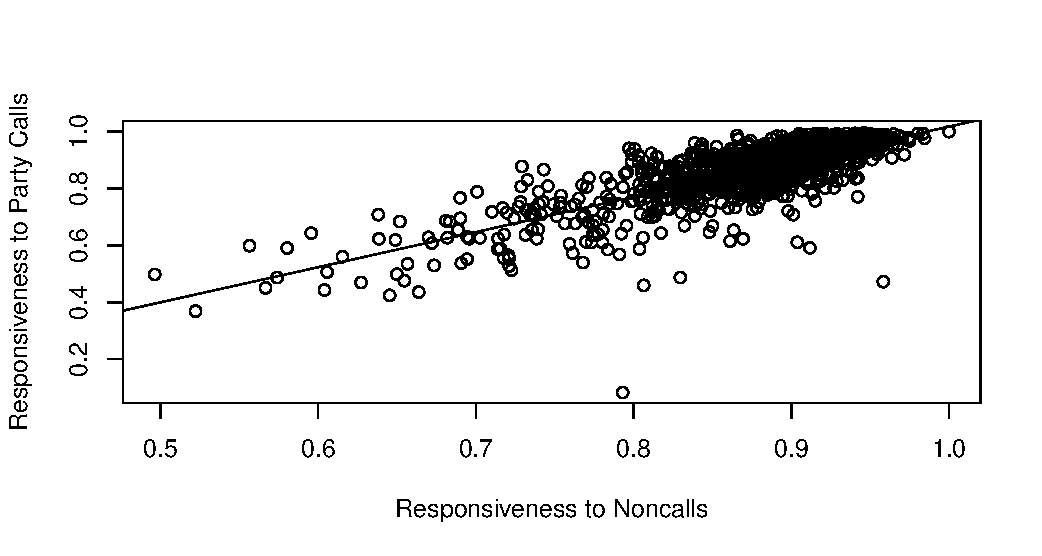
\includegraphics[width = \textwidth]{C:/Users/Ethan/Documents/GitHub/partycalls/plots/senate-old_dem_iv-dv_1.pdf}
\end{figure}

\begin{figure}[h]
	\caption{Main DV and Ideological Extremism - Senate Democrats, Old Algorithm}
	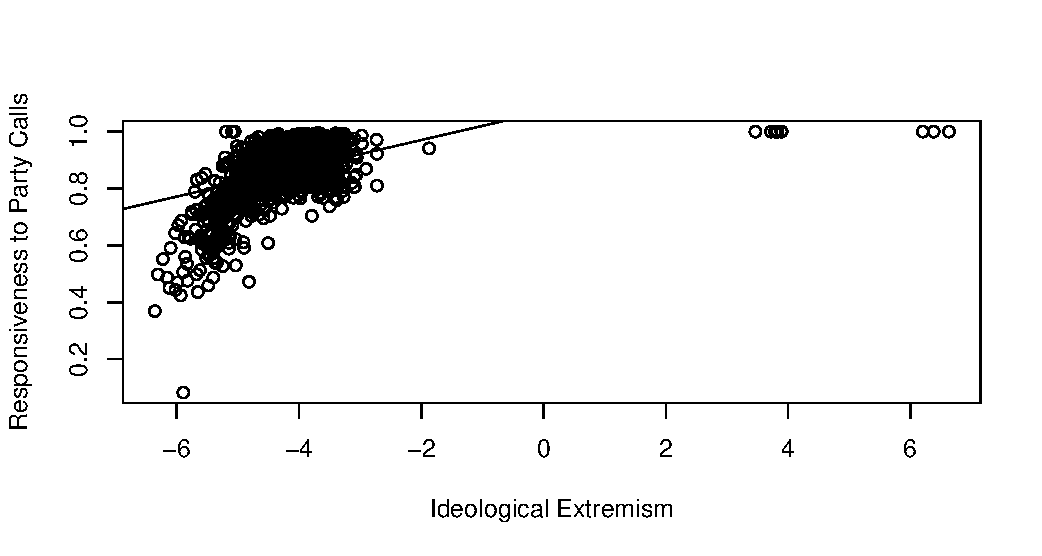
\includegraphics[width = \textwidth]{C:/Users/Ethan/Documents/GitHub/partycalls/plots/senate-old_dem_iv-dv_2.pdf}
\end{figure}

\begin{figure}[h]
	\caption{Main DV and IV - Senate Republicans, Old Algorithm}
	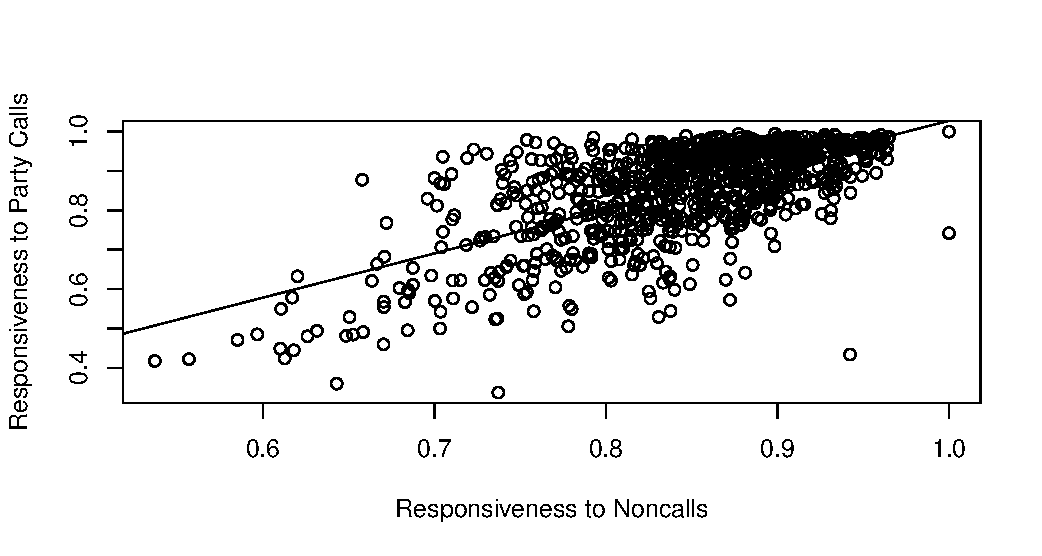
\includegraphics[width = \textwidth]{C:/Users/Ethan/Documents/GitHub/partycalls/plots/senate-old_rep_iv-dv_1.pdf}
\end{figure}

\begin{figure}[h]
	\caption{Main DV and Ideological Extremism - Senate Republicans, Old Algorithm}
	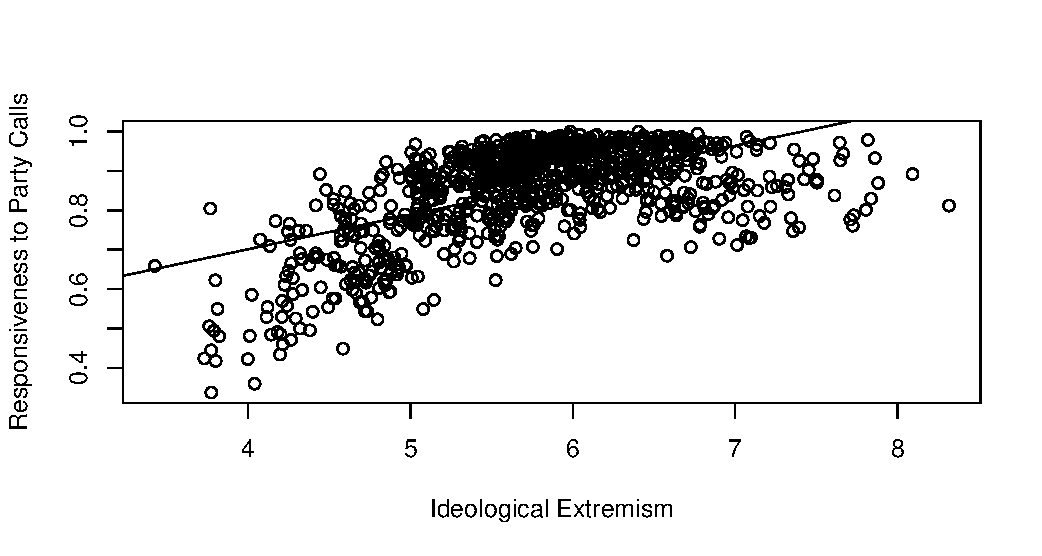
\includegraphics[width = \textwidth]{C:/Users/Ethan/Documents/GitHub/partycalls/plots/senate-old_rep_iv-dv_2.pdf}
\end{figure}

\begin{table}
	\begin{center}
		\caption{Old Senate Regression Table}
		\begin{tabular}{l c c c c }
			\hline
			& Democrats & Republicans & Democrats & Republicans \\
			\hline
			\textit{Distance from Floor Median}     & $0.040^{***}$  & $0.105^{***}$  &                &                \\
			& $(0.009)$      & $(0.008)$      &                &                \\
			\textit{Ideological Extremism}       &                &                & $0.056^{***}$  & $0.138^{***}$  \\
			&                &                & $(0.007)$      & $(0.007)$      \\
			\textit{Baseline Rate of Voting with Party}     & $0.993^{***}$  & $1.111^{***}$  & $0.907^{***}$  & $0.940^{***}$  \\
			& $(0.032)$      & $(0.040)$      & $(0.033)$      & $(0.036)$      \\
			\textit{Vote Share}                   & $-0.212^{*}$   & $-0.216$       & $-0.158$       & $-0.233$       \\
			& $(0.096)$      & $(0.204)$      & $(0.094)$      & $(0.185)$      \\
			\textit{Presidential Vote Share}             & $0.080$        & $-0.347$       & $0.120$        & $-0.404^{*}$   \\
			& $(0.125)$      & $(0.209)$      & $(0.122)$      & $(0.190)$      \\
			\textit{Vote Share $\times$ Presidential Vote Share} & $0.273$        & $0.576$        & $0.198$        & $0.586$        \\
			& $(0.192)$      & $(0.341)$      & $(0.188)$      & $(0.311)$      \\
			\textit{Up for Election}           & $-0.007$       & $-0.024^{***}$ & $-0.006$       & $-0.023^{***}$ \\
			& $(0.004)$      & $(0.006)$      & $(0.004)$      & $(0.005)$      \\
			\textit{Freshman}                      & $-0.017^{**}$  & $0.025^{**}$   & $-0.016^{**}$  & $0.026^{***}$  \\
			& $(0.006)$      & $(0.008)$      & $(0.006)$      & $(0.008)$      \\
			\textit{Retiree}                       & $0.001$        & $0.048^{***}$  & $-0.000$       & $0.042^{***}$  \\
			& $(0.008)$      & $(0.011)$      & $(0.008)$      & $(0.010)$      \\
			\textit{Seniority}                     & $-0.001$       & $-0.001$       & $-0.001$       & $0.000$        \\
			& $(0.001)$      & $(0.001)$      & $(0.001)$      & $(0.001)$      \\
			\textit{Party Leader}                       & $0.019$        & $0.019$        & $0.018$        & $0.021$        \\
			& $(0.010)$      & $(0.013)$      & $(0.010)$      & $(0.012)$      \\
			\textit{Committee Chair}                        & $0.012^{*}$    & $0.047^{***}$  & $0.010$        & $0.048^{***}$  \\
			& $(0.005)$      & $(0.008)$      & $(0.005)$      & $(0.007)$      \\
			\textit{Best Committee}               & $-0.001$       & $-0.001$       & $-0.001$       & $-0.001$       \\
			& $(0.001)$      & $(0.002)$      & $(0.001)$      & $(0.002)$      \\
			\textit{Power Committee}              & $-0.001$       & $-0.007$       & $-0.003$       & $-0.003$       \\
			& $(0.008)$      & $(0.010)$      & $(0.007)$      & $(0.009)$      \\
			\textit{South}                       & $-0.027^{***}$ & $0.021^{***}$  & $-0.020^{***}$ & $0.010$        \\
			& $(0.005)$      & $(0.006)$      & $(0.005)$      & $(0.006)$      \\
			\textit{African American}                          & $-0.000$       & $-0.116^{*}$   & $-0.004$       & $-0.041$       \\
			& $(0.028)$      & $(0.046)$      & $(0.027)$      & $(0.042)$      \\
			\textit{Female}                        & $0.008$        & $-0.016$       & $0.010$        & $-0.006$       \\
			& $(0.007)$      & $(0.012)$      & $(0.007)$      & $(0.011)$      \\
			\textit{Latino}                        & $0.009$        & $0.044$        & $0.013$        & $0.036$        \\
			& $(0.022)$      & $(0.030)$      & $(0.021)$      & $(0.027)$      \\
			\textit{Intercept}                   & $0.009$        & $-0.004$       & $0.048$        & $0.176$        \\
			& $(0.069)$      & $(0.129)$      & $(0.068)$      & $(0.118)$      \\
			\hline
			R$^2$                         & 0.699          & 0.587          & 0.709          & 0.658          \\
			Adj. R$^2$                    & 0.694          & 0.579          & 0.705          & 0.651          \\
			Num. obs.                     & 1037           & 929            & 1037           & 929            \\
			RMSE                          & 0.060          & 0.078          & 0.059          & 0.071          \\
			\hline
			\multicolumn{5}{l}{\scriptsize{$^{***}p<0.001$, $^{**}p<0.01$, $^*p<0.05$}}
		\end{tabular}
	\end{center}
\end{table}

\clearpage

\pagebreak

\subsection{Senator Year Data Summary Statistics}

% Table created by stargazer v.5.2 by Marek Hlavac, Harvard University. E-mail: hlavac at fas.harvard.edu
% Date and time: Mon, Jan 30, 2017 - 12:09:27
\begin{table}[!htbp] \centering 
	\caption{New Senator Year Data - Democrats} 
	\begin{tabular}{@{\extracolsep{5pt}}lccccc} 
		\\[-1.8ex]\hline 
		\hline \\[-1.8ex] 
		Statistic & \multicolumn{1}{c}{N} & \multicolumn{1}{c}{Mean} & \multicolumn{1}{c}{St. Dev.} & \multicolumn{1}{c}{Min} & \multicolumn{1}{c}{Max} \\ 
		\hline \\[-1.8ex]  
		maj & 1,039 & 0.632 & 0.473 & 0.000 & 1.000 \\ 
		pres\_vote\_share & 1,039 & 0.484 & 0.093 & 0.201 & 0.730 \\ 
		pres\_dem\_vote\_share & 1,039 & 0.484 & 0.093 & 0.201 & 0.730 \\ 
		vote\_share & 1,039 & 0.619 & 0.102 & 0.500 & 1.000 \\ 
		south & 1,039 & 0.237 & 0.425 & 0 & 1 \\ 
		south11 & 1,039 & 0.212 & 0.409 & 0 & 1 \\ 
		south13 & 1,039 & 0.237 & 0.425 & 0 & 1 \\ 
		south17 & 1,039 & 0.341 & 0.474 & 0 & 1 \\ 
		south\_dem & 1,039 & 0.237 & 0.425 & 0 & 1 \\ 
		leader & 1,039 & 0.084 & 0.277 & 0 & 1 \\ 
		chair & 1,039 & 0.208 & 0.406 & 0 & 1 \\ 
		best\_committee & 1,039 & 12.253 & 2.758 & 0 & 15 \\ 
		power\_committee & 1,037 & 0.728 & 0.445 & 0 & 1 \\ 
		up\_for\_reelection & 1,039 & 0.334 & 0.472 & 0 & 1 \\ 
		freshman & 1,039 & 0.328 & 0.470 & 0 & 1 \\ 
		superfreshman & 1,039 & 0.011 & 0.102 & 0 & 1 \\ 
		seniority & 1,039 & 6.770 & 4.916 & 1 & 26 \\ 
		senate\_seniority & 1,039 & 2.594 & 1.629 & 1 & 9 \\ 
		retiree & 1,039 & 0.050 & 0.218 & 0 & 1 \\ 
		afam & 1,039 & 0.005 & 0.069 & 0 & 1 \\ 
		female & 1,039 & 0.084 & 0.277 & 0 & 1 \\ 
		latino & 1,039 & 0.007 & 0.082 & 0 & 1 \\ 
		gingrich\_senator & 1,039 & 0.000 & 0.000 & 0 & 0 \\ 
		votes & 1,039 & 742.239 & 204.558 & 28 & 1,311 \\ 
		drop & 1,039 & 0.000 & 0.000 & 0 & 0 \\ 
		\hline
		party\_free\_ideal\_point $ p < 0.01 $ & 1,039 & $-$0.793 & 0.520 & $-$2.037 & 1.389 \\  
		pirate100 $ p < 0.01 $ & 1,039 & 82.629 & 11.671 & 6.250 & 100.000 \\ 
		pfrate100 $ p < 0.01 $ & 1,039 & 84.053 & 10.057 & 19.095 & 100.000 \\ 
		ideological\_extremism $ p < 0.01 $ & 1,039 & 0.793 & 0.520 & $-$1.389 & 2.037 \\ 
		\hline
		party\_free\_ideal\_point $ p < 0.05 $ & 1,039 & $-$0.786 & 0.529 & $-$2.059 & 1.568 \\ 
		pirate100 $ p < 0.05 $ & 1,039 & 82.391 & 11.120 & 12.000 & 100.000 \\  
		pfrate100 $ p < 0.05 $ & 1,039 & 84.214 & 9.973 & 20.000 & 100.000 \\ 
		ideological\_extremism $ p < 0.05 $ & 1,039 & 0.786 & 0.529 & $-$1.568 & 2.059 \\ 
		\hline \\[-1.8ex] 
	\end{tabular} 
\end{table} 

% Table created by stargazer v.5.2 by Marek Hlavac, Harvard University. E-mail: hlavac at fas.harvard.edu
% Date and time: Mon, Jan 30, 2017 - 12:09:29
\begin{table}[!htbp] \centering 
	\caption{New Senator Year Data - Republicans $ p < 0.01 $} 
	\begin{tabular}{@{\extracolsep{5pt}}lccccc} 
		\\[-1.8ex]\hline 
		\hline \\[-1.8ex] 
		Statistic & \multicolumn{1}{c}{N} & \multicolumn{1}{c}{Mean} & \multicolumn{1}{c}{St. Dev.} & \multicolumn{1}{c}{Min} & \multicolumn{1}{c}{Max} \\ 
		\hline \\[-1.8ex] 
		maj & 950 & 0.464 & 0.489 & 0.000 & 1.000 \\ 
		pres\_vote\_share & 950 & 0.562 & 0.085 & 0.310 & 0.780 \\ 
		pres\_dem\_vote\_share & 950 & 0.438 & 0.085 & 0.220 & 0.690 \\ 
		vote\_share & 950 & 0.605 & 0.094 & 0.500 & 1.000 \\ 
		south & 950 & 0.286 & 0.452 & 0 & 1 \\ 
		south11 & 950 & 0.229 & 0.421 & 0 & 1 \\ 
		south13 & 950 & 0.286 & 0.452 & 0 & 1 \\ 
		south17 & 950 & 0.338 & 0.473 & 0 & 1 \\ 
		south\_dem & 950 & 0.000 & 0.000 & 0 & 0 \\ 
		leader & 950 & 0.117 & 0.321 & 0 & 1 \\ 
		chair & 950 & 0.155 & 0.362 & 0 & 1 \\ 
		best\_committee & 950 & 12.327 & 2.621 & 0 & 15 \\ 
		power\_committee & 949 & 0.724 & 0.447 & 0 & 1 \\ 
		up\_for\_reelection & 950 & 0.332 & 0.471 & 0 & 1 \\ 
		freshman & 950 & 0.385 & 0.487 & 0 & 1 \\ 
		superfreshman & 950 & 0.005 & 0.072 & 0 & 1 \\ 
		seniority & 950 & 5.682 & 4.163 & 1 & 24 \\ 
		senate\_seniority & 950 & 2.236 & 1.373 & 1 & 8 \\ 
		retiree & 950 & 0.067 & 0.251 & 0 & 1 \\ 
		afam & 950 & 0.003 & 0.056 & 0 & 1 \\ 
		female & 950 & 0.048 & 0.215 & 0 & 1 \\ 
		latino & 950 & 0.007 & 0.086 & 0 & 1 \\ 
		gingrich\_senator & 950 & 0.197 & 0.398 & 0 & 1 \\ 
		votes & 950 & 726.227 & 187.300 & 41 & 1,291 \\ 
		drop & 950 & 0.000 & 0.000 & 0 & 0 \\ 
		\hline
		party\_free\_ideal\_point $ p < 0.01 $ & 950 & 0.872 & 0.590 & $-$1.189 & 2.664 \\ 
		pirate100 $ p < 0.01 $ & 950 & 83.255 & 12.598 & 32.990 & 100.000 \\ 
		pfrate100 $ p < 0.01 $ & 950 & 81.881 & 10.173 & 41.923 & 100.000 \\ 
		ideological\_extremism $ p < 0.01 $ & 950 & 0.872 & 0.590 & $-$1.189 & 2.664 \\  
		\hline \\[-1.8ex] 
	\end{tabular} 
\end{table} 

% Table created by stargazer v.5.2 by Marek Hlavac, Harvard University. E-mail: hlavac at fas.harvard.edu
% Date and time: Mon, Jan 30, 2017 - 13:42:54
\begin{table}[!htbp] \centering 
	\caption{New Senator Year Data - Republicans $ p < 0.01 $} 
	\begin{tabular}{@{\extracolsep{5pt}}lccccc} 
		\\[-1.8ex]\hline 
		\hline \\[-1.8ex] 
		Statistic & \multicolumn{1}{c}{N} & \multicolumn{1}{c}{Mean} & \multicolumn{1}{c}{St. Dev.} & \multicolumn{1}{c}{Min} & \multicolumn{1}{c}{Max} \\ 
		\hline \\[-1.8ex]  
		maj & 951 & 0.464 & 0.489 & 0.000 & 1.000 \\ 
		pres\_vote\_share & 951 & 0.562 & 0.085 & 0.310 & 0.780 \\ 
		pres\_dem\_vote\_share & 951 & 0.438 & 0.085 & 0.220 & 0.690 \\ 
		vote\_share & 951 & 0.605 & 0.094 & 0.500 & 1.000 \\ 
		south & 951 & 0.286 & 0.452 & 0 & 1 \\ 
		south11 & 951 & 0.229 & 0.421 & 0 & 1 \\ 
		south13 & 951 & 0.286 & 0.452 & 0 & 1 \\ 
		south17 & 951 & 0.338 & 0.473 & 0 & 1 \\ 
		south\_dem & 951 & 0.000 & 0.000 & 0 & 0 \\ 
		leader & 951 & 0.117 & 0.321 & 0 & 1 \\ 
		chair & 951 & 0.155 & 0.362 & 0 & 1 \\ 
		best\_committee & 951 & 12.314 & 2.650 & 0 & 15 \\ 
		power\_committee & 949 & 0.724 & 0.447 & 0 & 1 \\ 
		up\_for\_reelection & 951 & 0.332 & 0.471 & 0 & 1 \\ 
		freshman & 951 & 0.386 & 0.487 & 0 & 1 \\ 
		superfreshman & 951 & 0.005 & 0.072 & 0 & 1 \\ 
		seniority & 951 & 5.677 & 4.163 & 1 & 24 \\ 
		senate\_seniority & 951 & 2.234 & 1.373 & 1 & 8 \\ 
		retiree & 951 & 0.067 & 0.251 & 0 & 1 \\ 
		afam & 951 & 0.003 & 0.056 & 0 & 1 \\ 
		female & 951 & 0.048 & 0.215 & 0 & 1 \\ 
		latino & 951 & 0.007 & 0.086 & 0 & 1 \\ 
		gingrich\_senator & 951 & 0.198 & 0.398 & 0 & 1 \\ 
		votes & 951 & 725.506 & 188.520 & 40 & 1,291 \\ 
		drop & 951 & 0.000 & 0.000 & 0 & 0 \\ 
		\hline
		party\_free\_ideal\_point $ p < 0.05 $ & 951 & 0.863 & 0.604 & $-$1.291 & 2.679 \\ 
		pirate100 $ p < 0.05 $ & 951 & 81.747 & 11.728 & 35.714 & 100.000 \\ 
		pfrate100 $ p < 0.05 $ & 951 & 81.940 & 10.277 & 41.515 & 100.000 \\ 
		ideological\_extremism $ p < 0.05 $ & 951 & 0.863 & 0.604 & $-$1.291 & 2.679 \\ 
		\hline \\[-1.8ex] 
	\end{tabular} 
\end{table} 

% Table created by stargazer v.5.2 by Marek Hlavac, Harvard University. E-mail: hlavac at fas.harvard.edu
% Date and time: Mon, Jan 30, 2017 - 12:09:30
\begin{table}[!htbp] \centering 
	\caption{New Senator Year Data - Majority Caucus} 
	\begin{tabular}{@{\extracolsep{5pt}}lccccc} 
		\\[-1.8ex]\hline 
		\hline \\[-1.8ex] 
		Statistic & \multicolumn{1}{c}{N} & \multicolumn{1}{c}{Mean} & \multicolumn{1}{c}{St. Dev.} & \multicolumn{1}{c}{Min} & \multicolumn{1}{c}{Max} \\ 
		\hline \\[-1.8ex] 
		maj & 1,049 & 1.000 & 0.000 & 1 & 1 \\ 
		pres\_vote\_share & 1,049 & 0.506 & 0.101 & 0.201 & 0.780 \\ 
		pres\_dem\_vote\_share & 1,049 & 0.462 & 0.094 & 0.201 & 0.730 \\ 
		vote\_share & 1,049 & 0.613 & 0.100 & 0.500 & 1.000 \\ 
		south & 1,049 & 0.268 & 0.443 & 0 & 1 \\ 
		south11 & 1,049 & 0.232 & 0.422 & 0 & 1 \\ 
		south13 & 1,049 & 0.268 & 0.443 & 0 & 1 \\ 
		south17 & 1,049 & 0.345 & 0.476 & 0 & 1 \\ 
		south\_dem & 1,049 & 0.148 & 0.355 & 0 & 1 \\ 
		leader & 1,049 & 0.096 & 0.295 & 0 & 1 \\ 
		chair & 1,049 & 0.329 & 0.470 & 0 & 1 \\ 
		best\_committee & 1,049 & 12.266 & 2.734 & 0 & 15 \\ 
		power\_committee & 1,047 & 0.719 & 0.450 & 0 & 1 \\ 
		up\_for\_reelection & 1,049 & 0.323 & 0.468 & 0 & 1 \\ 
		freshman & 1,049 & 0.391 & 0.488 & 0 & 1 \\ 
		superfreshman & 1,049 & 0.006 & 0.075 & 0 & 1 \\ 
		seniority & 1,049 & 6.076 & 4.591 & 1 & 26 \\ 
		senate\_seniority & 1,049 & 2.370 & 1.517 & 1 & 9 \\ 
		retiree & 1,049 & 0.051 & 0.219 & 0 & 1 \\ 
		afam & 1,049 & 0.002 & 0.044 & 0 & 1 \\ 
		female & 1,049 & 0.064 & 0.245 & 0 & 1 \\ 
		latino & 1,049 & 0.009 & 0.092 & 0 & 1 \\ 
		gingrich\_senator & 1,049 & 0.087 & 0.282 & 0 & 1 \\ 
		votes & 1,049 & 748.442 & 201.319 & 28 & 1,311 \\ 
		drop & 1,049 & 0.000 & 0.000 & 0 & 0 \\ 
		\hline
		party\_free\_ideal\_point $ p < 0.01 $ & 1,049 & $-$0.064 & 0.905 & $-$2.005 & 2.351 \\ 
		pirate100 $ p < 0.01 $ & 1,049 & 83.477 & 11.495 & 40.625 & 100.000 \\ 
		pfrate100 $ p < 0.01 $ & 1,049 & 84.420 & 9.743 & 36.663 & 100.000 \\ 
		ideological\_extremism $ p < 0.01 $ & 1,049 & 0.741 & 0.523 & $-$1.389 & 2.351 \\ 
		\hline
		party\_free\_ideal\_point $ p < 0.05 $ & 1,049 & $-$0.060 & 0.904 & $-$1.966 & 2.379 \\ 
		pirate100 $ p < 0.05 $ & 1,049 & 83.165 & 11.006 & 35.190 & 100.000 \\ 
		pfrate100 $ p < 0.05 $ & 1,049 & 84.553 & 9.649 & 38.983 & 100.000 \\ 
		ideological\_extremism $ p < 0.05 $ & 1,049 & 0.733 & 0.531 & $-$1.568 & 2.379 \\ 
		\hline \\[-1.8ex] 
	\end{tabular} 
\end{table} 

% Table created by stargazer v.5.2 by Marek Hlavac, Harvard University. E-mail: hlavac at fas.harvard.edu
% Date and time: Mon, Jan 30, 2017 - 12:09:32
\begin{table}[!htbp] \centering 
	\caption{New Senator Year Data - Minority Caucus, $ p < 0.01 $} 
	\begin{tabular}{@{\extracolsep{5pt}}lccccc} 
		\\[-1.8ex]\hline 
		\hline \\[-1.8ex] 
		Statistic & \multicolumn{1}{c}{N} & \multicolumn{1}{c}{Mean} & \multicolumn{1}{c}{St. Dev.} & \multicolumn{1}{c}{Min} & \multicolumn{1}{c}{Max} \\ 
		\hline \\[-1.8ex] 
		maj & 842 & 0.000 & 0.000 & 0 & 0 \\ 
		pres\_vote\_share & 842 & 0.538 & 0.091 & 0.284 & 0.754 \\ 
		pres\_dem\_vote\_share & 842 & 0.461 & 0.090 & 0.246 & 0.690 \\ 
		vote\_share & 842 & 0.611 & 0.098 & 0.500 & 1.000 \\ 
		south & 842 & 0.251 & 0.434 & 0 & 1 \\ 
		south11 & 842 & 0.205 & 0.404 & 0 & 1 \\ 
		south13 & 842 & 0.251 & 0.434 & 0 & 1 \\ 
		south17 & 842 & 0.333 & 0.471 & 0 & 1 \\ 
		south\_dem & 842 & 0.097 & 0.297 & 0 & 1 \\ 
		leader & 842 & 0.102 & 0.303 & 0 & 1 \\ 
		chair & 842 & 0.000 & 0.000 & 0 & 0 \\ 
		best\_committee & 842 & 12.315 & 2.626 & 0 & 15 \\ 
		power\_committee & 841 & 0.734 & 0.442 & 0 & 1 \\ 
		up\_for\_reelection & 842 & 0.344 & 0.475 & 0 & 1 \\ 
		freshman & 842 & 0.311 & 0.463 & 0 & 1 \\ 
		superfreshman & 842 & 0.012 & 0.108 & 0 & 1 \\ 
		seniority & 842 & 6.416 & 4.544 & 1 & 24 \\ 
		senate\_seniority & 842 & 2.474 & 1.506 & 1 & 8 \\ 
		retiree & 842 & 0.070 & 0.255 & 0 & 1 \\ 
		afam & 842 & 0.007 & 0.084 & 0 & 1 \\ 
		female & 842 & 0.064 & 0.245 & 0 & 1 \\ 
		latino & 842 & 0.006 & 0.077 & 0 & 1 \\ 
		gingrich\_senator & 842 & 0.093 & 0.290 & 0 & 1 \\ 
		votes & 842 & 731.044 & 197.372 & 41 & 1,291 \\ 
		drop & 842 & 0.000 & 0.000 & 0 & 0 \\ 
		\hline
		party\_free\_ideal\_point $ p < 0.01 $ & 842 & 0.082 & 1.100 & $-$2.037 & 2.664 \\ 
		pirate100 $ p < 0.01 $ & 842 & 82.034 & 12.716 & 6.250 & 100.000 \\ 
		pfrate100 $ p < 0.01 $ & 842 & 80.797 & 10.469 & 19.095 & 100.000 \\ 
		ideological\_extremism $ p < 0.01 $ & 842 & 0.930 & 0.593 & $-$1.189 & 2.664 \\  
		\hline \\[-1.8ex] 
	\end{tabular} 
\end{table} 

% Table created by stargazer v.5.2 by Marek Hlavac, Harvard University. E-mail: hlavac at fas.harvard.edu
% Date and time: Mon, Jan 30, 2017 - 13:42:58
\begin{table}[!htbp] \centering 
	\caption{New Senator Year Data - Minority Caucus, $ p < 0.05 $} 
	\begin{tabular}{@{\extracolsep{5pt}}lccccc} 
		\\[-1.8ex]\hline 
		\hline \\[-1.8ex] 
		Statistic & \multicolumn{1}{c}{N} & \multicolumn{1}{c}{Mean} & \multicolumn{1}{c}{St. Dev.} & \multicolumn{1}{c}{Min} & \multicolumn{1}{c}{Max} \\ 
		\hline \\[-1.8ex] 
		congress & 843 & 102.507 & 5.780 & 93 & 112 \\ 
		icpsrLegis & 843 & 18,105.650 & 12,780.780 & 52 & 94,659 \\ 
		class & 843 & 2.030 & 0.808 & 1 & 3 \\ 
		maj & 843 & 0.000 & 0.000 & 0 & 0 \\ 
		pres\_vote\_share & 843 & 0.538 & 0.091 & 0.284 & 0.754 \\ 
		pres\_dem\_vote\_share & 843 & 0.461 & 0.090 & 0.246 & 0.690 \\ 
		vote\_share & 843 & 0.611 & 0.098 & 0.500 & 1.000 \\ 
		south & 843 & 0.250 & 0.433 & 0 & 1 \\ 
		south11 & 843 & 0.205 & 0.404 & 0 & 1 \\ 
		south13 & 843 & 0.250 & 0.433 & 0 & 1 \\ 
		south17 & 843 & 0.332 & 0.471 & 0 & 1 \\ 
		south\_dem & 843 & 0.097 & 0.297 & 0 & 1 \\ 
		leader & 843 & 0.102 & 0.303 & 0 & 1 \\ 
		chair & 843 & 0.000 & 0.000 & 0 & 0 \\ 
		best\_committee & 843 & 12.300 & 2.659 & 0 & 15 \\ 
		power\_committee & 841 & 0.734 & 0.442 & 0 & 1 \\ 
		up\_for\_reelection & 843 & 0.345 & 0.476 & 0 & 1 \\ 
		freshman & 843 & 0.312 & 0.464 & 0 & 1 \\ 
		superfreshman & 843 & 0.012 & 0.108 & 0 & 1 \\ 
		seniority & 843 & 6.409 & 4.545 & 1 & 24 \\ 
		senate\_seniority & 843 & 2.472 & 1.506 & 1 & 8 \\ 
		retiree & 843 & 0.070 & 0.255 & 0 & 1 \\ 
		afam & 843 & 0.007 & 0.084 & 0 & 1 \\ 
		female & 843 & 0.064 & 0.245 & 0 & 1 \\ 
		latino & 843 & 0.006 & 0.077 & 0 & 1 \\ 
		gingrich\_senator & 843 & 0.094 & 0.292 & 0 & 1 \\ 
		votes & 843 & 730.224 & 198.685 & 40 & 1,291 \\ 
		drop & 843 & 0.000 & 0.000 & 0 & 0 \\ 
		\hline
		party\_free\_ideal\_point $ p < 0.05 $ & 843 & 0.079 & 1.102 & $-$2.059 & 2.679 \\ 
		pirate100 $ p < 0.05 $ & 843 & 80.443 & 11.709 & 12.000 & 100.000 \\ 
		pfrate100 $ p < 0.05 $ & 843 & 80.868 & 10.614 & 20.000 & 100.000 \\ 
		ideological\_extremism $ p < 0.05 $ & 843 & 0.920 & 0.612 & $-$1.291 & 2.679 \\ 
		\hline \\[-1.8ex] 
	\end{tabular} 
\end{table}

\pagebreak

\subsection{Plots and Regressions of Main DV and IVs}

\begin{table}[ht]
	\begin{center}
		\caption{Senate $ p < 0.01 $ Algorithm}
		\begin{tabular}{l c c c c }
			\hline
			& Democrats & Democrats & Republicans & Republicans \\
			\hline
			pfrate100              & $0.87^{***}$ &               & $0.99^{***}$ &               \\
			& $(0.02)$     &               & $(0.02)$     &               \\
			ideological\_extremism &              & $11.47^{***}$ &              & $11.58^{***}$ \\
			&              & $(0.60)$      &              & $(0.58)$      \\
			(Intercept)            & $9.31^{***}$ & $73.53^{***}$ & $2.44$       & $73.16^{***}$ \\
			& $(2.01)$     & $(0.57)$      & $(2.00)$     & $(0.61)$      \\
			\hline
			R$^2$                  & 0.57         & 0.26          & 0.64         & 0.29          \\
			Adj. R$^2$             & 0.56         & 0.26          & 0.63         & 0.29          \\
			Num. obs.              & 1039         & 1039          & 950          & 950           \\
			RMSE                   & 7.70         & 10.03         & 7.61         & 10.59         \\
			\hline
			\multicolumn{5}{l}{\scriptsize{$^{***}p<0.001$, $^{**}p<0.01$, $^*p<0.05$}}
		\end{tabular}
	\end{center}
\end{table}

\begin{figure}[h]
	\caption{Main DV and IV - Senate Democrats, $p < 0.01$}
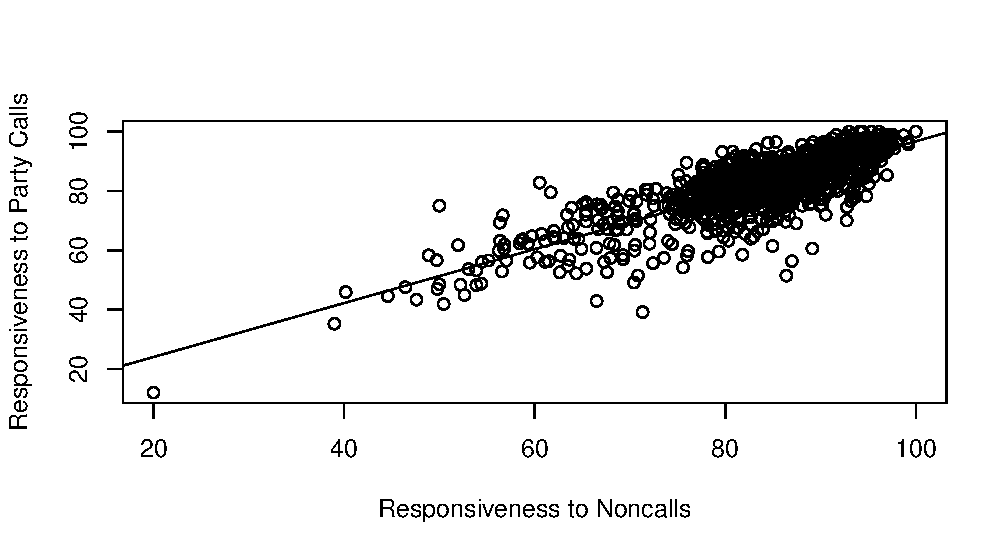
\includegraphics[width = \textwidth]{C:/Users/Ethan/Documents/GitHub/partycalls/plots/senate-emIRT_dem_iv-dv_1.pdf}
\end{figure}

\begin{figure}[h]
	\caption{Main DV and Ideological Extremism - Democrats, $p < 0.01$}
	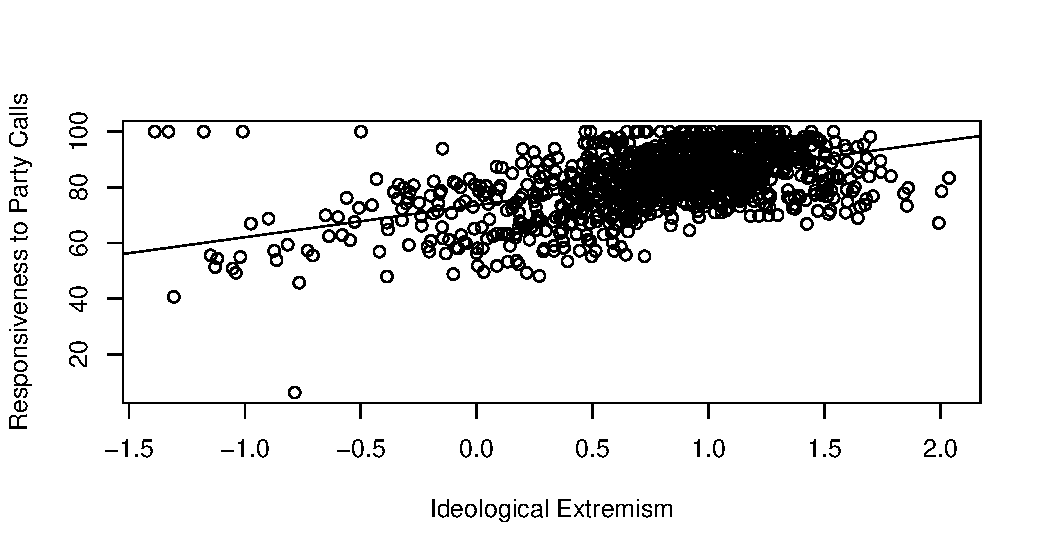
\includegraphics[width = \textwidth]{C:/Users/Ethan/Documents/GitHub/partycalls/plots/senate-emIRT_dem_iv-dv_2.pdf}
\end{figure}

\begin{figure}[h]
\caption{Main DV and IV - Senate Republicans, $p < 0.01$}
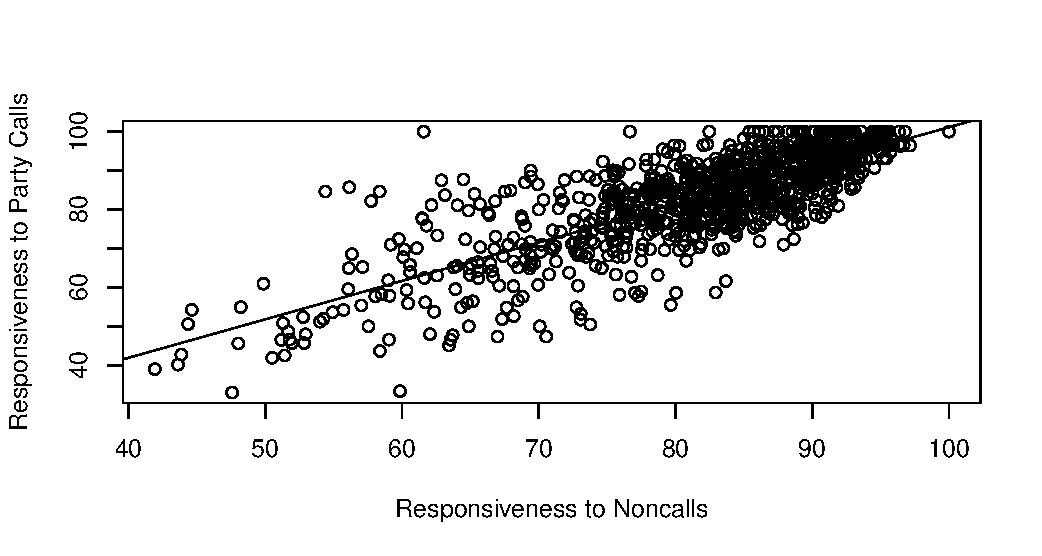
\includegraphics[width = \textwidth]{C:/Users/Ethan/Documents/GitHub/partycalls/plots/senate-emIRT_rep_iv-dv_1.pdf}
\end{figure}

\begin{figure}[h]
	\caption{Main DV and Ideological Extremism - Senate Republicans, $p < 0.01$}
	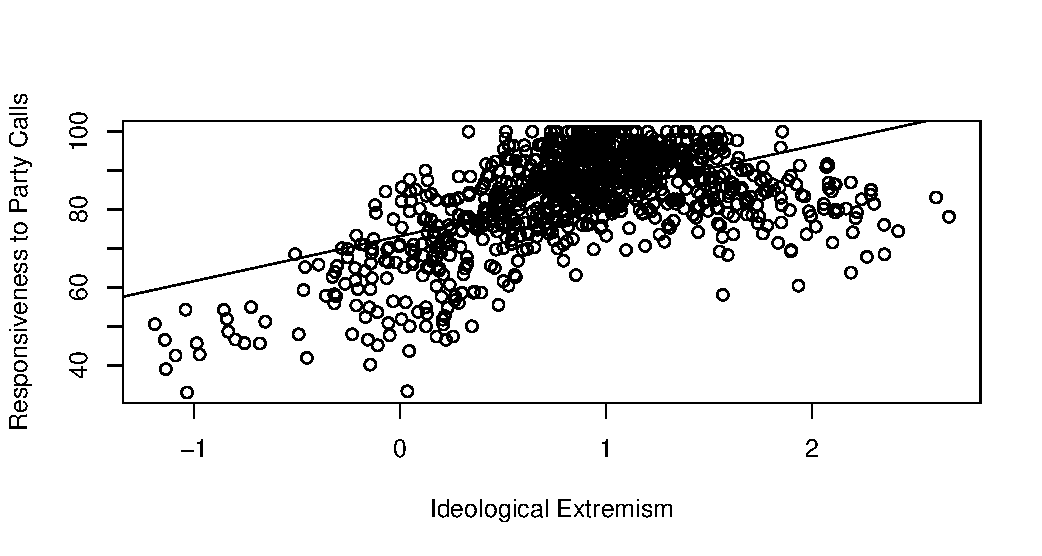
\includegraphics[width = \textwidth]{C:/Users/Ethan/Documents/GitHub/partycalls/plots/senate-emIRT_rep_iv-dv_2.pdf}
\end{figure}

\begin{table}
	\begin{center}
		\caption{Senate $ p < 0.05 $ Algorithm}
		\begin{tabular}{l c c c c }
			\hline
			& Democrats & Democrats & Republicans & Republicans \\
			\hline
			pfrate100              & $0.91^{***}$ &               & $0.93^{***}$ &               \\
			& $(0.02)$     &               & $(0.02)$     &               \\
			ideological\_extremism &              & $12.39^{***}$ &              & $10.64^{***}$ \\
			&              & $(0.53)$      &              & $(0.53)$      \\
			(Intercept)            & $5.80^{***}$ & $72.66^{***}$ & $5.85^{**}$  & $72.56^{***}$ \\
			& $(1.70)$     & $(0.50)$      & $(1.79)$     & $(0.56)$      \\
			\hline
			R$^2$                  & 0.67         & 0.35          & 0.66         & 0.30          \\
			Adj. R$^2$             & 0.66         & 0.35          & 0.66         & 0.30          \\
			Num. obs.              & 1039         & 1039          & 951          & 951           \\
			RMSE                   & 6.44         & 8.99          & 6.85         & 9.81          \\
			\hline
			\multicolumn{5}{l}{\scriptsize{$^{***}p<0.001$, $^{**}p<0.01$, $^*p<0.05$}}
		\end{tabular}
	\end{center}
\end{table}

\begin{figure}[h]
	\caption{Main DV and IV - Senate Democrats, $p < 0.05$}
	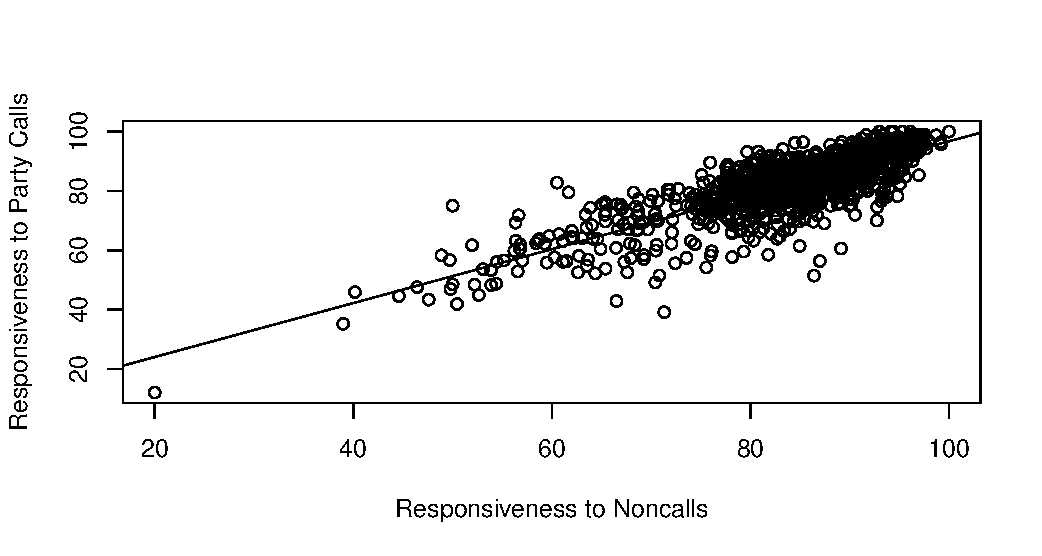
\includegraphics[width = \textwidth]{C:/Users/Ethan/Documents/GitHub/partycalls/plots/senate-p_05_dem_iv-dv_1.pdf}
\end{figure}

\begin{figure}[h]
	\caption{Main DV and Ideological Extremism - Senate Democrats, $p < 0.05$}
	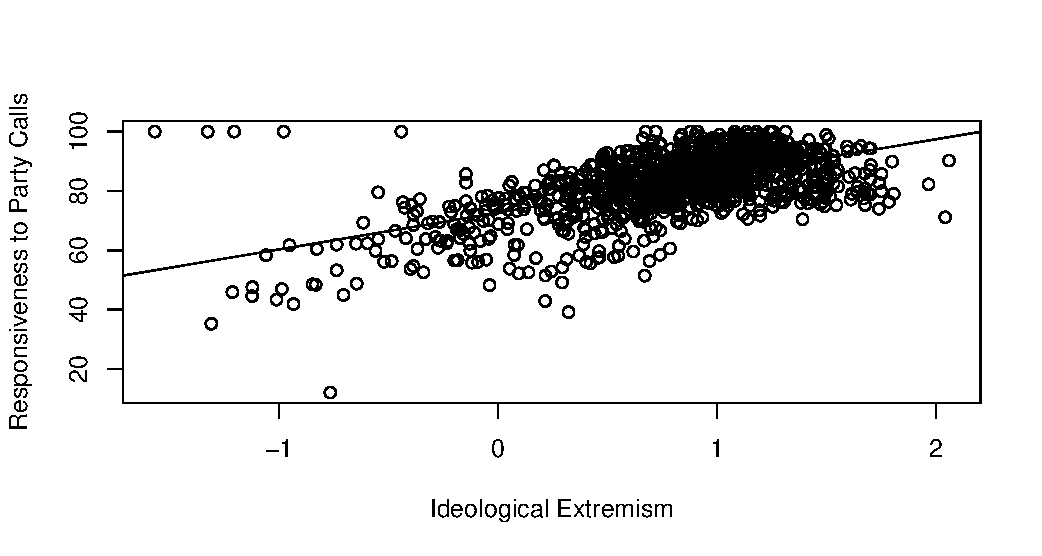
\includegraphics[width = \textwidth]{C:/Users/Ethan/Documents/GitHub/partycalls/plots/senate-p_05_dem_iv-dv_2.pdf}
\end{figure}

\begin{figure}[h]
	\caption{Main DV and IV - Senate Republicans, $p < 0.5$}
	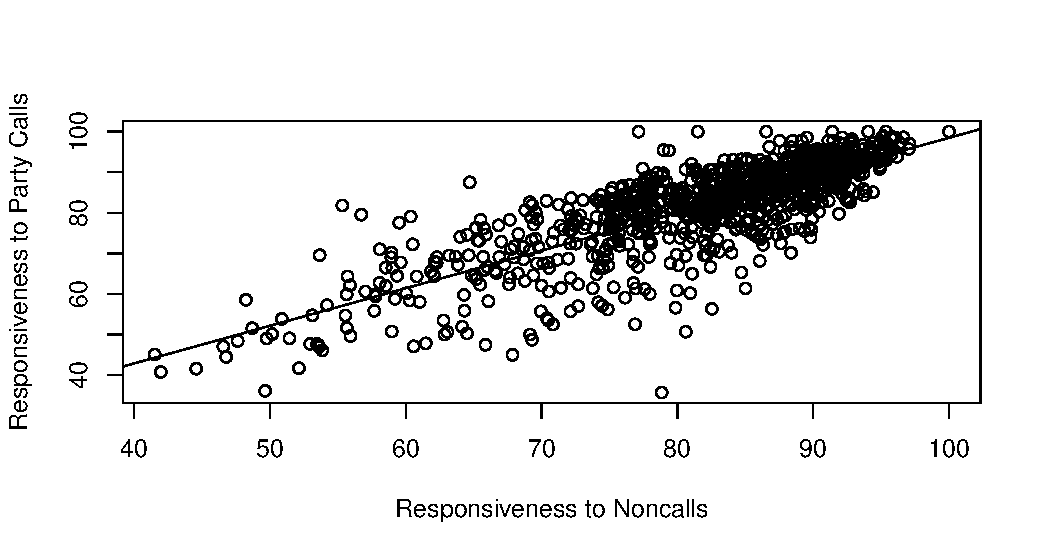
\includegraphics[width = \textwidth]{C:/Users/Ethan/Documents/GitHub/partycalls/plots/senate-p_05_rep_iv-dv_1.pdf}
\end{figure}

\begin{figure}[h]
	\caption{Main DV and Ideological Extremism - Senate Republicans, $p < 0.05$}
	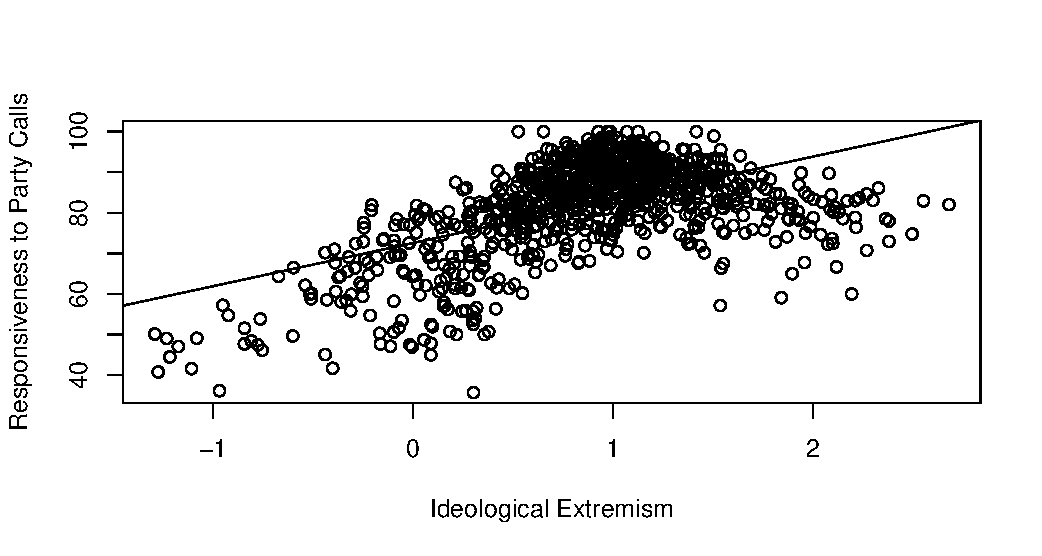
\includegraphics[width = \textwidth]{C:/Users/Ethan/Documents/GitHub/partycalls/plots/senate-p_05_rep_iv-dv_2.pdf}
\end{figure}











\end{document}